\chapter{ Analyse et Sp\'{e}cifications besoins }
\section{Introduction}


Cette partie consiste en une \'{e}tape analytique dans laquelle nous allons
recenser et factoriser les besoins des utilisateurs de l'application. Ceci est
fortement li\'{e} \`{a} l'\'{e}tude pr\'{e}alable men\'{e}e au
Cours du premier chapitre.
Pour ce faire cette phase doit r\'{e}pondre aux questions suivantes :
Quels sont les besoins fonctionnels de l'application ?
Quelles sont les contraintes qui doivent \^{e}tre prises en consid\'{e}ration?

   \section{ Les acteurs du syst\`{e}me }
C'est une entit\'{e} externe qui agit sur le syst\`{e}me (op\'{e}rateur, autre syst\`{e}me,
\ldots{}).Il peut consulter
Ou modifier l'\'{e}tat du syst\`{e}me.
En r\'{e}ponse \`{a} l'action d'un acteur, le syst\`{e}me fournit un service qui
correspond \`{a} son besoin.
Le principal acteur de syst\`{e}me :
\begin{itemize}
\item{  \textbf{L'administrateur :} entit\'{e} externe principale. Son r\^{o}le est qui a le droit de
g\'{e}rer un projet (cr\'{e}er, modifier, supprimer).
Aussi son r\^{o}le et de g\'{e}rer l'affectation des taches aux membres
correspondants.
}

\item{ \textbf{Le membre : } entit\'{e} externe secondaire, il peut se connecter pour consulter la
t\^{a}che en cours que l'administrateur lui a effectu\'{e} et la marquer comme
termin\'{e}e ou non.
}
\end{itemize}


\section{ Sp\'{e}cifications besoins}

  \subsection{Besoins fonctionnels}

Le besoin primordiale de notre application et de permettre à l’administrateur
de « Cherchini » de gérer les projets et ceci consiste à :

\subsubsection{G\'{e}rer les projets}

\begin{itemize}
\item{La cr\'{e}ation d’un projet.}
\item{La modification d'un projet.}
\item{La suppression d'un projet.}
\item{Consulter les projets et les t\^{a}che et les d\'{e}tails correspondants.}
\item{Affecter les membres correspondants \`{a} chaque projet.}
\end{itemize}

\subsubsection{G\'{e}rer les t\^{a}che}

\begin{itemize}
\item{La cr\'{e}ation d'une t\^{a}che.}
\item{La modification d'une t\^{a}che.}
\item{La suppression d'une t\^{a}che.}
\item{Consulter les t\^{a}che et les d\'{e}tails correspondants.}
\item{Affecter le membre correspondant \`{a} chaque t\^{a}che.}
\end{itemize}

\subsubsection{G\'{e}rer les membres}

\begin{itemize}
\item{La cr\'{e}ation d'un membre.}
\item{La modification d'un membre.}
\item{La suppression d'un membre.}
\item{Consulter les membres et leurs d\'{e}tails correspondants.}
\item{Affecter les membres correspondants \`{a} chaque projet.}
\end{itemize}

\subsubsection{G\'{e}rer les clients}

\begin{itemize}
\item{La cr\'{e}ation d'un .}
\item{La modification d'un client.}
\item{La suppression d'un client.}
\item{Consulter les clients et leurs d\'{e}tails correspondants.}
\end{itemize}

\subsubsection{
Suivre le d\'{e}roulement des projets}

\begin{itemize}
\item{ Suivre le travail des \'{e}quipes en consultant le diagramme Gantt pour chaque projet.}
\item{Consulter les rapports des co\^{u}ts et les dur\'{e}es selon les projets et les clients   .}
\item{Consulter la carte g\'{e}ographique des g\'{e}olocalisations des  .}
\end{itemize}

  \subsection{Besoins non fonctionnels}
Les besoins non fonctionnels sp\'{e}cifient les propri\'{e}t\'{e}s du syst\`{e}me afin de
garantir la Coh\'{e}rence, la confidentialit\'{e} et l'int\'{e}grit\'{e} des donn\'{e}es.
Le syst\`{e}me doit \^{e}tre fiable: la validit\'{e} de l`application.
R\'{e}utilisabilit\'{e}: aptitude de site \`{a} \^{e}tre utilis\'{e} en tout ou en partie dans de
nouvelles applications.

\subsubsection{La performance d'ex\'{e}cution}

Le temps d'ex\'{e}cution du syst\`{e}me doit \^{e}tre minimal pour ne pas g\^{e}ner
l'utilisateur. Ce temps d\'{e}pend de la complexit\'{e} du code impl\'{e}ment\'{e}, du
serveur d'application utilis\'{e}, du d\'{e}bit de la ligne de connexion et de la
conception de la base de donn\'{e}es.

\subsubsection{La s\'{e}curit\'{e}}

Le syst\`{e}me doit respecter un niveau de s\'{e}curit\'{e} \'{e}lev\'{e} afin de garantir la
confidentialit\'{e} de l'acc\`{e}s des membres

\subsubsection{L'ergonomie }

L'interface de cette application doit \^{e}tre ergonome, conviviale et voire m\^{e}me
apte \`{a} aider l'utilisateur \`{a} mieux g\'{e}rer son espace de travail.






\section{ Diagramme de cas d'utilisation g\'{e}n\'{e}rale }
Le diagramme de cas d'utilisation permet de d\'{e}crire l'interaction entre
l'acteur et le syst\`{e}me.
Le cas d'utilisation est une description des interactions qui vont permettre \`{a}
l'acteur d'atteindre son objectif en utilisant le syst\`{e}me. Un acteur et un cas
d'utilisation sont mis en relation par une association repr\'{e}sent\'{e}e par une
ligne.
Le but principal du diagramme du cas d'utilisation est de d\'{e}finir le syst\`{e}me
du point de vue des utilisateurs et de d\'{e}finir les limites pr\'{e}cises du syst\`{e}me en
utilisant une notation tr\`{e}s simple






\FloatBarrier
\begin{figure}[H]
\center
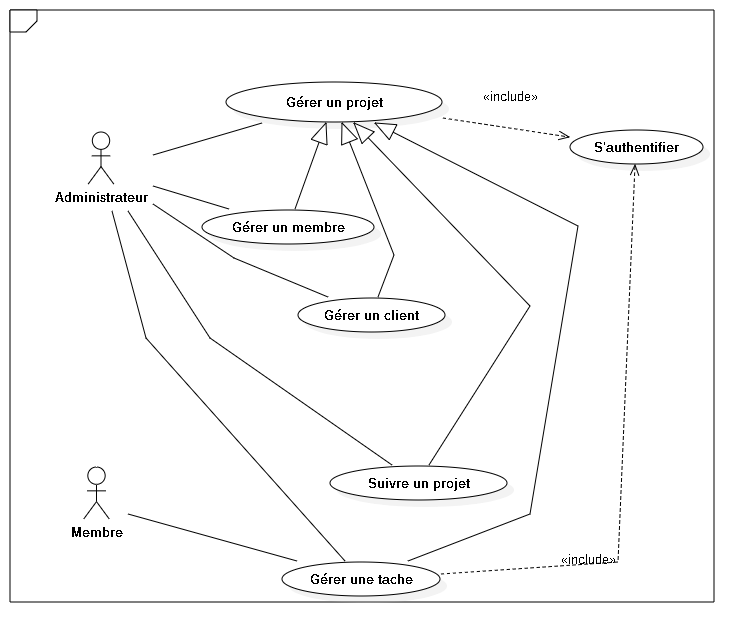
\includegraphics[width=13cm,height=10cm]{./figures/ucG.png}
\caption{Diagramme de cas d'utilisation g\'{e}n\'{e}rale.}

\end{figure}
\FloatBarrier


\section{ Etude m\'{e}thodologique }



  \subsection{Choix de la   m\'{e}thodologie}

  Dans la plupart des projets, on a besoin de suivre un processus qui d\'{e}finit
QUI fait QUOI, QUAND et COMMENT pour \^{e}tre capable de :

\begin{itemize}
\item{Atteindre un certain objectif.}
\item{Construire des mod\`{e}les d'un ou de plusieurs syst\`{e}mes.}
\item{G\'{e}rer le cycle de vie du projet de A \`{a} Z.}
\item{Organiser le projet}
\item{G\'{e}rer les risques}
\item{Obtenir de mani\`{e}re r\'{e}p\'{e}titive des produits de qualit\'{e} constante}
\end{itemize}

Le choix entre une m\'{e}thode et une autre, d\'{e}pend de la nature du projet et de sa taille. Pour des
projets de petite taille et dont le domaine est ma\^{\i}tris\'{e}, par exemple, un cycle de vie en cascade
s'av\`{e}re largement su Sant. Lorsqu'il s'agit d'un projet o\`{u} les donn\'{e}es ne sont pas r\'{e}unies d\`{e}s le
d\'{e}part, o\`{u} les besoins sont incomplets voire floues, il faut s'orienter vers une m\'{e}thode it\'{e}rative
ou orient\'{e}es prototypes.
Parmi les m\'{e}thodes it\'{e}ratives, nous pouvons distinguer les m\'{e}thodes agiles largement utilis\'{e}es
de nos jours \`{a} travers le monde. Une m\'{e}thode agile est men\'{e}e dans un esprit collaboratif et
s'adapte aux approches incr\'{e}mentales. Elle engendre des produits de haute qualit\'{e} tout en tenant
compte de l'\'{e}volution des besoins du client.
La nature de projet qui doit \^{e}tre \'{e}volutif et dont tous les besoins n'ont pas encore \'{e}t\'{e}
totalement identit\'{e}s, nous a orient\'{e}es vers une m\'{e}thode de type agile et plus particuli\`{e}rement
SCRUM.
  \subsection{Pr\'{e}sentation de la m\'{e}thodologie SCRUM}
Scrum signifie m\^{e}l\'{e}e au rugby. Il exploite les valeurs et l'esprit du rugby et les adapte aux
projets de d\'{e}veloppement. Comme le pack lors d'un ballon port\'{e} au rugby, l'\'{e}quipe charg\'{e}e du
d\'{e}veloppement de travaille de fa\c{c}on collective, soud\'{e}e vers un objectif pr\'{e}cis. Comme un demi
de m\^{e}l\'{e}e, le ScrumMaster est le responsable du projet qui oriente les membres de l'\'{e}quipe dans
la bonne direction, assure l'environnement de travail et chercher \`{a} am\'{e}liorer la productivit\'{e} et
le savoir faire de don \'{e}quipe.
Scrum se base sur la th\'{e}orie du contr\^{o}le empirique de processus. L'empirisme mentionne que
les connaissances proviennent de l'exp\'{e}rience et d'une prise de d\'{e}cision bas\'{e}e sur des faits
connus. Scrum utilise une approche it\'{e}rative et incr\'{e}mentale pour optimiser la pr\'{e}dictibilit\'{e} et
contr\^{o}ler le risque.
\begin{figure}[H]
\center
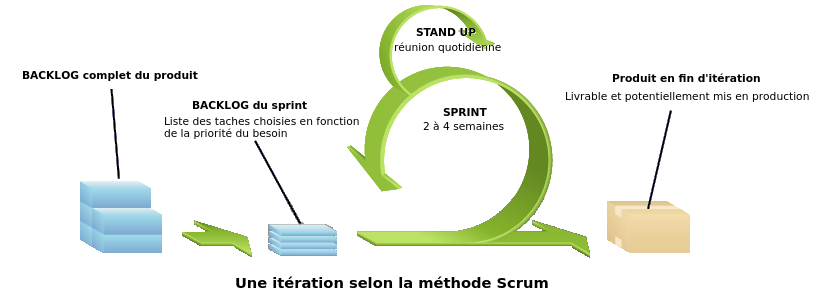
\includegraphics[width=10cm,height=6cm]{./figures/scrum.png}
\caption{Logo de Cherchini.}

\end{figure}

Comme nous pouvons le remarquer dans cette figure, pour mettre en place la m\'{e}thode
SCRUM, il faut tout d'abord d\'{e}finir les diff\'{e}rentes fonctionnalit\'{e}s de notre application qui
forment le Backlog du produit. Ensuite, nous proc\'{e}dons \`{a} la planification du sprint pour d\'{e}finir
le plan d\'{e}taill\'{e} d'une it\'{e}ration. Les sprints durent g\'{e}n\'{e}ralement deux \`{a} quatre semaines. Durant
un sprint, il y a toujours des r\'{e}unions quotidiennes entre les diff\'{e}rents collaborateurs du projet
pour pr\'{e}senter l'\'{e}tat d'avancement des diff\'{e}rentes t\^{a}ches en cours, les difficult\'{e}s rencontr\'{e}es
ainsi que les t\^{a}ches restantes \`{a} r\'{e}aliser. Une fois le produit partiel est pr\^{e}t, nous v\'{e}rifions la
conformit\'{e} de ce qui a \'{e}t\'{e} fait durant le sprint et nous pouvons alors l'am\'{e}liorer en proc\'{e}dant \`{a}
l'\'{e}tape de r\'{e}trospective.


\subsection{Planning du projet}

\FloatBarrier

Le tableau suivant résume les étapes que nous avons suivies






\begin{table}

\begin{tabular}{|l|l|l|}
\hline
Backlog                       & Sprint                                                                                                                                                            & Durée                        \\
\hline
                              & \begin{tabular}[c]{@{}l@{}}Recherche sur les nouvelles technologies\\~qu’on va utiliser \end{tabular}                                                             & 3 Semaines                   \\
\hline
                              & Formation sur les langages                                                                                                                                        & 3 Semaines                   \\
\hline
                              & \begin{tabular}[c]{@{}l@{}}Rédaction du chapitre présentation\\~de cadre générale \end{tabular}                                                                   & 2 jours                      \\
\hline
                              & \multirow{3}{*}{\begin{tabular}[c]{@{}l@{}}Création des diagrammes (Diagramme de classe,\\~Diagramme de séquence, Diagramme \\de cas d’utilisation)\end{tabular}} & \multirow{3}{*}{3 Semaines}  \\
\cline{1-1}
Etape Initiale                &                                                                                                                                                                   &                              \\
\cline{1-1}
                              &                                                                                                                                                                   &                              \\
\hline
                              & Rédaction du chapitre spécification des besoins                                                                                                                   & 2 jours                      \\
\hline
\multicolumn{3}{|l|}{Réunion}                                                                                                                                                                                                    \\
\hline
                              & \multirow{3}{*}{\begin{tabular}[c]{@{}l@{}}Création des premières interfaces de l’application\\(Gestion des membres ,clients ,projet ,tâches ) \end{tabular}}     & \multirow{3}{*}{1 Semaine}   \\
\cline{1-1}
                              &                                                                                                                                                                   &                              \\
\cline{1-1}
                              &                                                                                                                                                                   &                              \\
\hline
                              & Rédaction du chapitre conception                                                                                                                                  & 2 jours                      \\
\hline
                              & Création diagramme de Gantt                                                                                                                                       & 1 jour                       \\
\hline
Etape 2                       & \begin{tabular}[c]{@{}l@{}}Maintenance et test de la fonctionnalité \\gestion de projet\end{tabular}                                                              & 2 jours                      \\
\hline
                              & \begin{tabular}[c]{@{}l@{}}Développement de l’interface Gannt \\et de la carte géographique\end{tabular}                                                          & 2 jours                      \\
\hline
\multicolumn{3}{|l|}{Réunion}                                                                                                                                                                                                    \\
\hline
\multirow{2}{*}{Etape 3~ ~~}  & Développement de~l’interface membre                                                                                                                               & 1 Semaine                    \\
\cline{2-3}
                              & Développement de la partie~Authentification                                                                                                                       & 1 Semaine                    \\
\hline
\multicolumn{3}{|l|}{Réunion}                                                                                                                                                                                                    \\
\hline
\multirow{2}{*}{Etape 4}      & Développement de la partie~ETL                                                                                                                                    & 3 jours                      \\
\cline{2-3}
                              & \begin{tabular}[c]{@{}l@{}}Ajouter les rapports à l’interface\\~administrateur\end{tabular}                                                                       & 1 jour                       \\
\hline
\multicolumn{3}{|l|}{Réunion}                                                                                                                                                                                                    \\
\hline
\multirow{3}{*}{Etape finale} & \begin{tabular}[c]{@{}l@{}}Dernières retouches sur le design \\de l’application\end{tabular}                                                                      & 3 jours                      \\
\cline{2-3}
                              & Mises à jour du                                                                                                                                                   & \multirow{2}{*}{3 jours}     \\
\cline{2-2}
                              & rapport                                                                                                                                                           &                              \\
\hline
\multicolumn{1}{l}{}          & \multicolumn{1}{l}{}                                                                                                                                              & \multicolumn{1}{l}{}
\end{tabular}
\centering
\caption{Planning du projet}
\end{table}






%\begin{figure}[!h]
%\center
%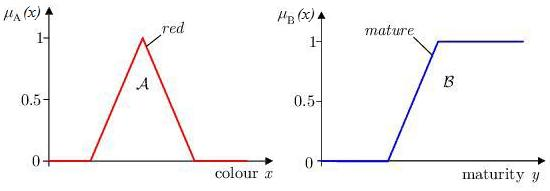
\includegraphics[width=10cm,height=6cm]{Relation.png}
%\caption{Titre de la Figure.}
%
%\end{figure}

%~~~~Bla bla bla exempe d'une liste:
%\begin{itemize}
%\item{}
%\item{}
%\item{}
%\item{}
%\end{itemize}

